\documentclass[a4,12pt]{article}

% 畫圖
\usepackage{tikz}
\usetikzlibrary{automata,positioning,arrows}


% 排版
% \usepackage{enumerate}
% \newlist{steps}{enumerate}{1}
% \setlist[steps, 1]{label = Step \arabic*:}

% 中文插件
\usepackage{fontspec}
\usepackage{xeCJK}
\setCJKmainfont{Heiti TC}


% 插入圖片 using \includegraphics[scale = 1]{name.jpg}
\usepackage{graphicx}
\graphicspath{{./picture/}}
\usepackage{float} %设置图片浮动位置的宏包
\usepackage{subfigure}

% \usepackage[]{caption}
% \capto

\usepackage{multicol}

\title{Computer Graphics Hw 4} 
\author{賴柏勛 00957126}

\begin{document}
    \maketitle
    \section{操作方法}

    7: 開關平行光

    \&: 控制平行光位置,營造日升日落

    8: 將平行光的顏色隨機變成另外一個

    *: 更改平行光強度

    9: 開關點光源

    [: 將點光源的顏色隨機變成另外一個

    \{: 更改點光源強度

    0: 開關機器人的聚光燈

    ]: 更改聚光燈的 cutoff angle

    \}: 更改聚光燈的強度 
    \newpage
    \section{畫面展示}
    \begin{multicols}{2}

        沒開燈的畫面

        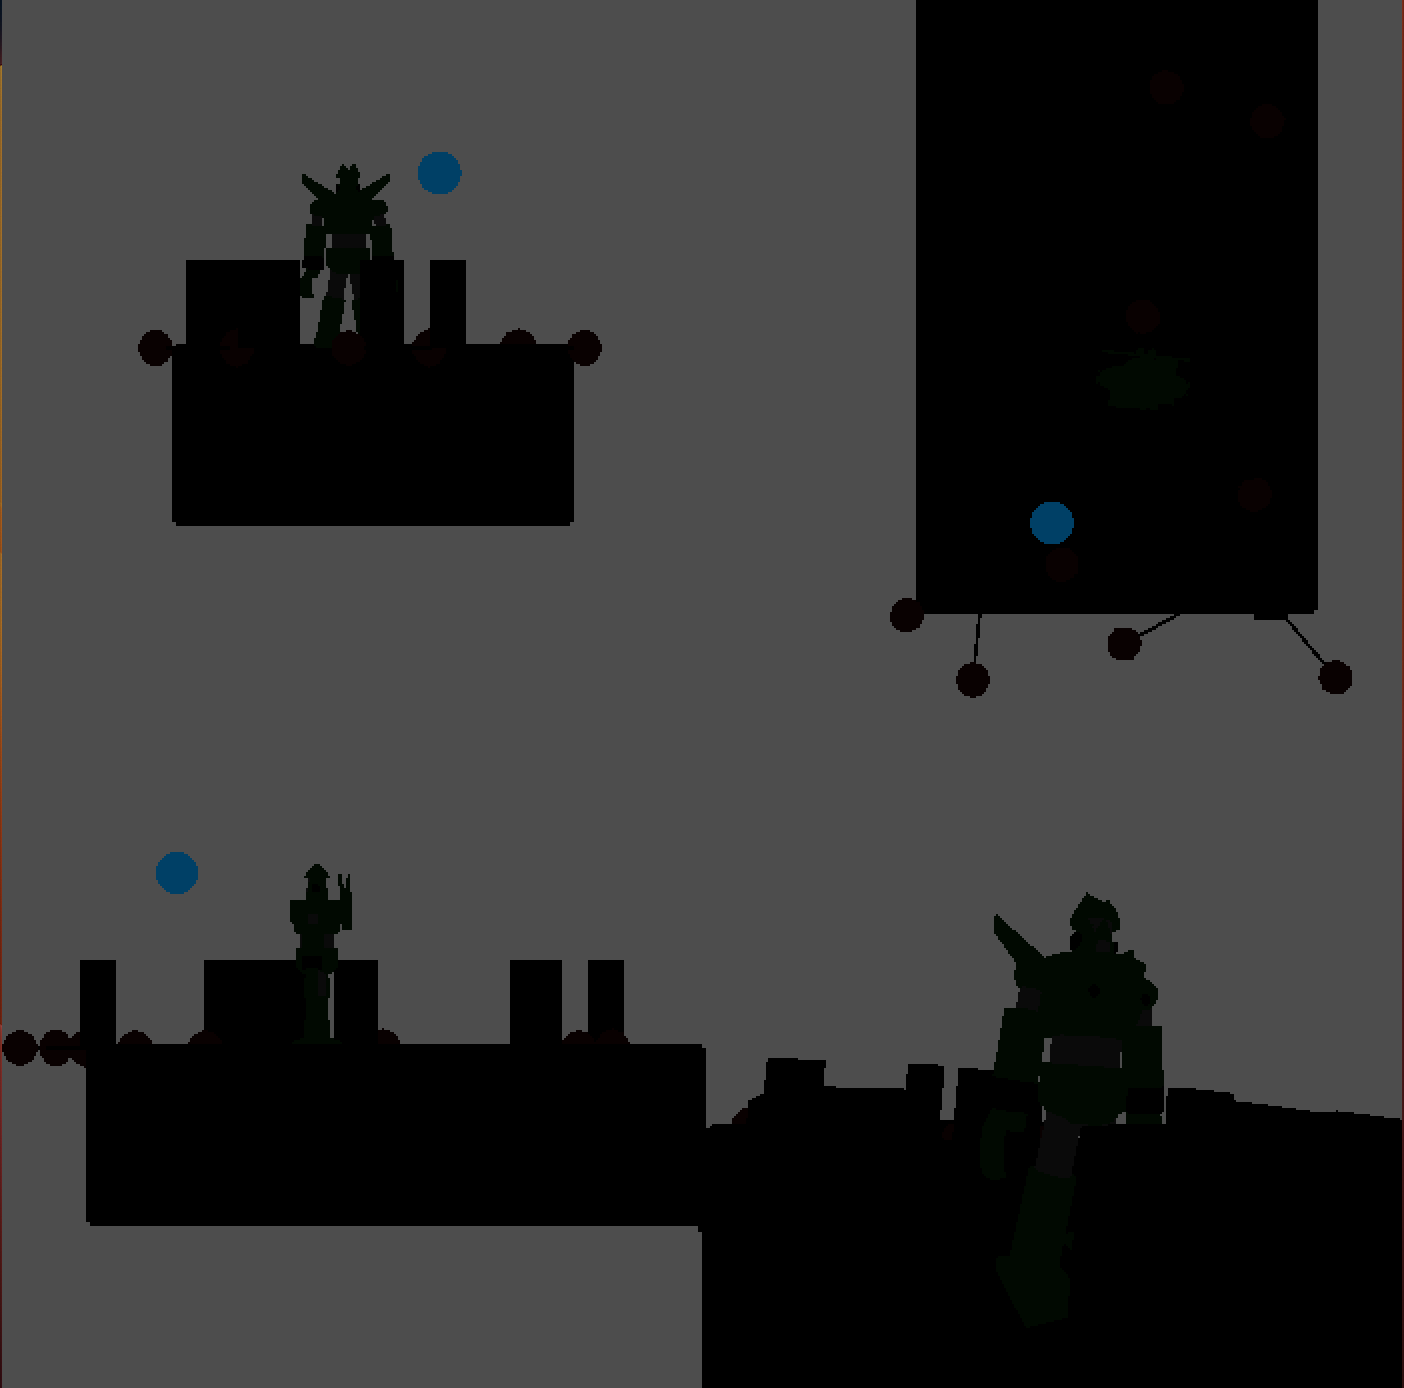
\includegraphics[scale=0.28]{pic.png}

        \columnbreak

        開平行光的畫面

        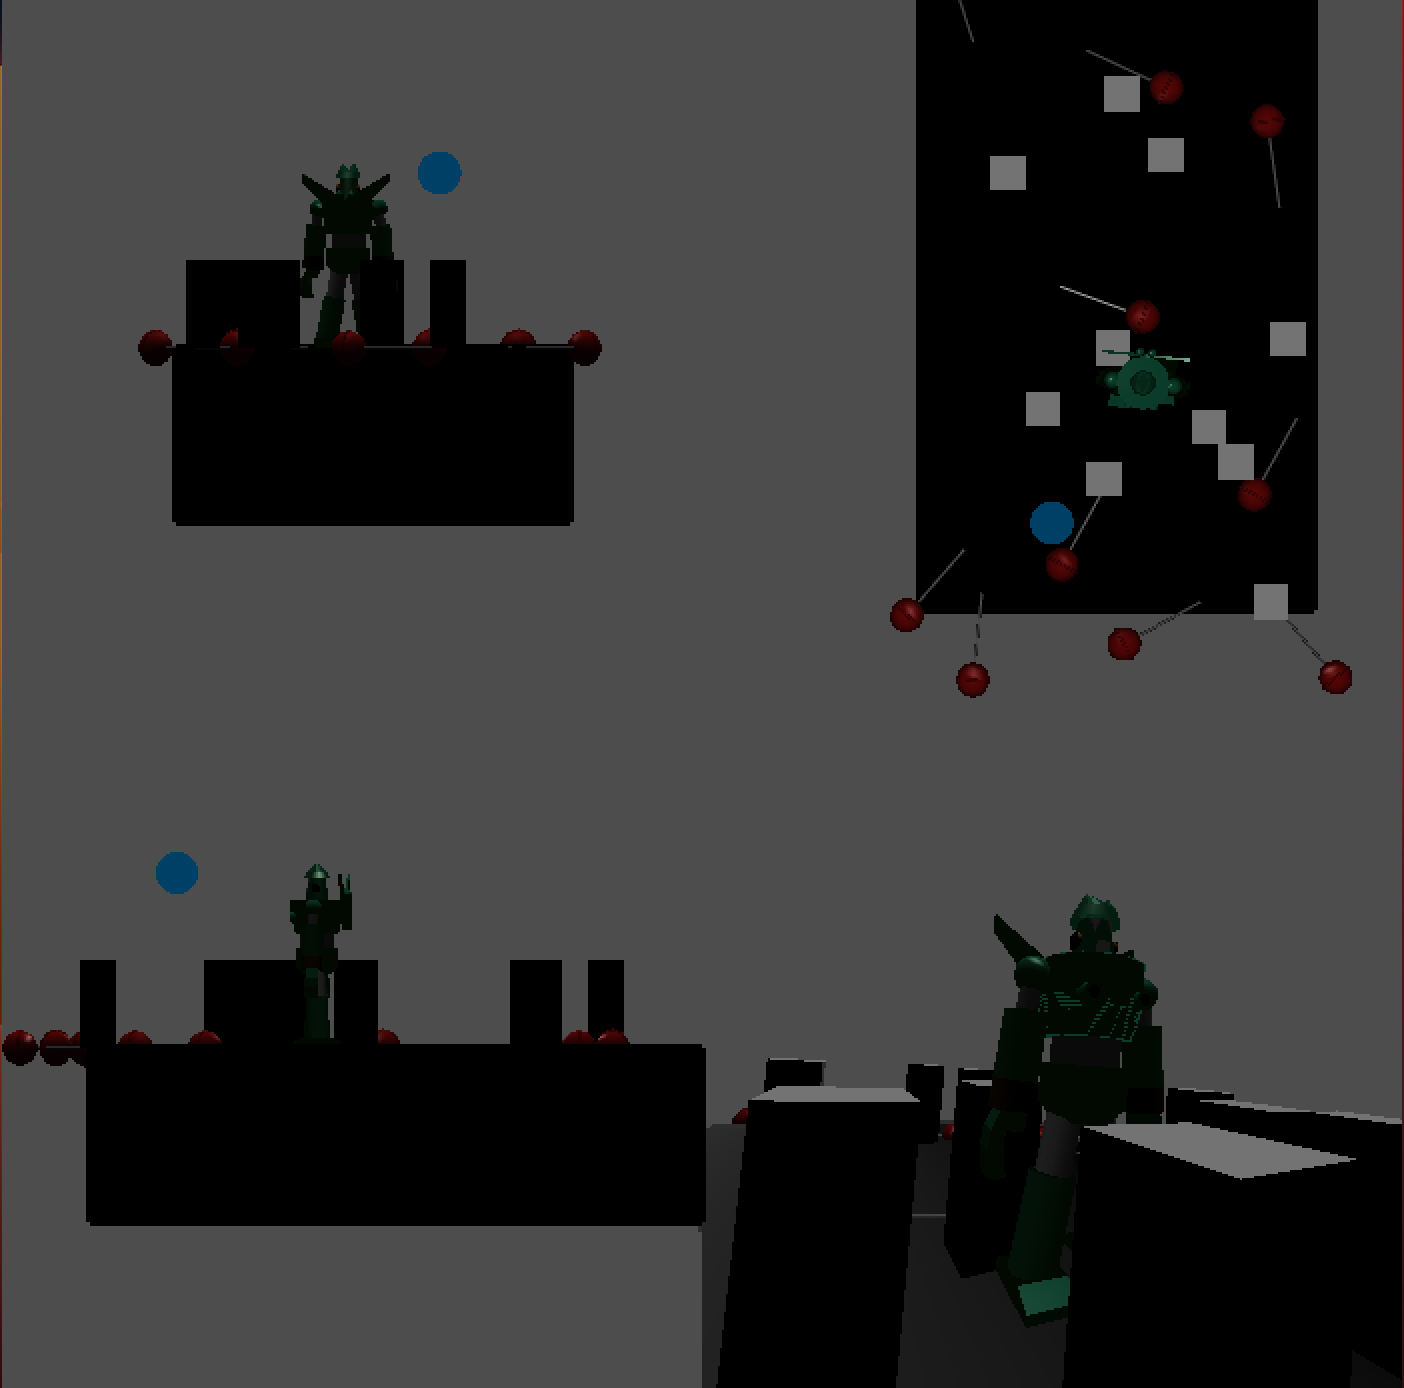
\includegraphics[scale=0.28]{pic1.png}

    \end{multicols}
    \begin{multicols}{2}

        開點光源的畫面

        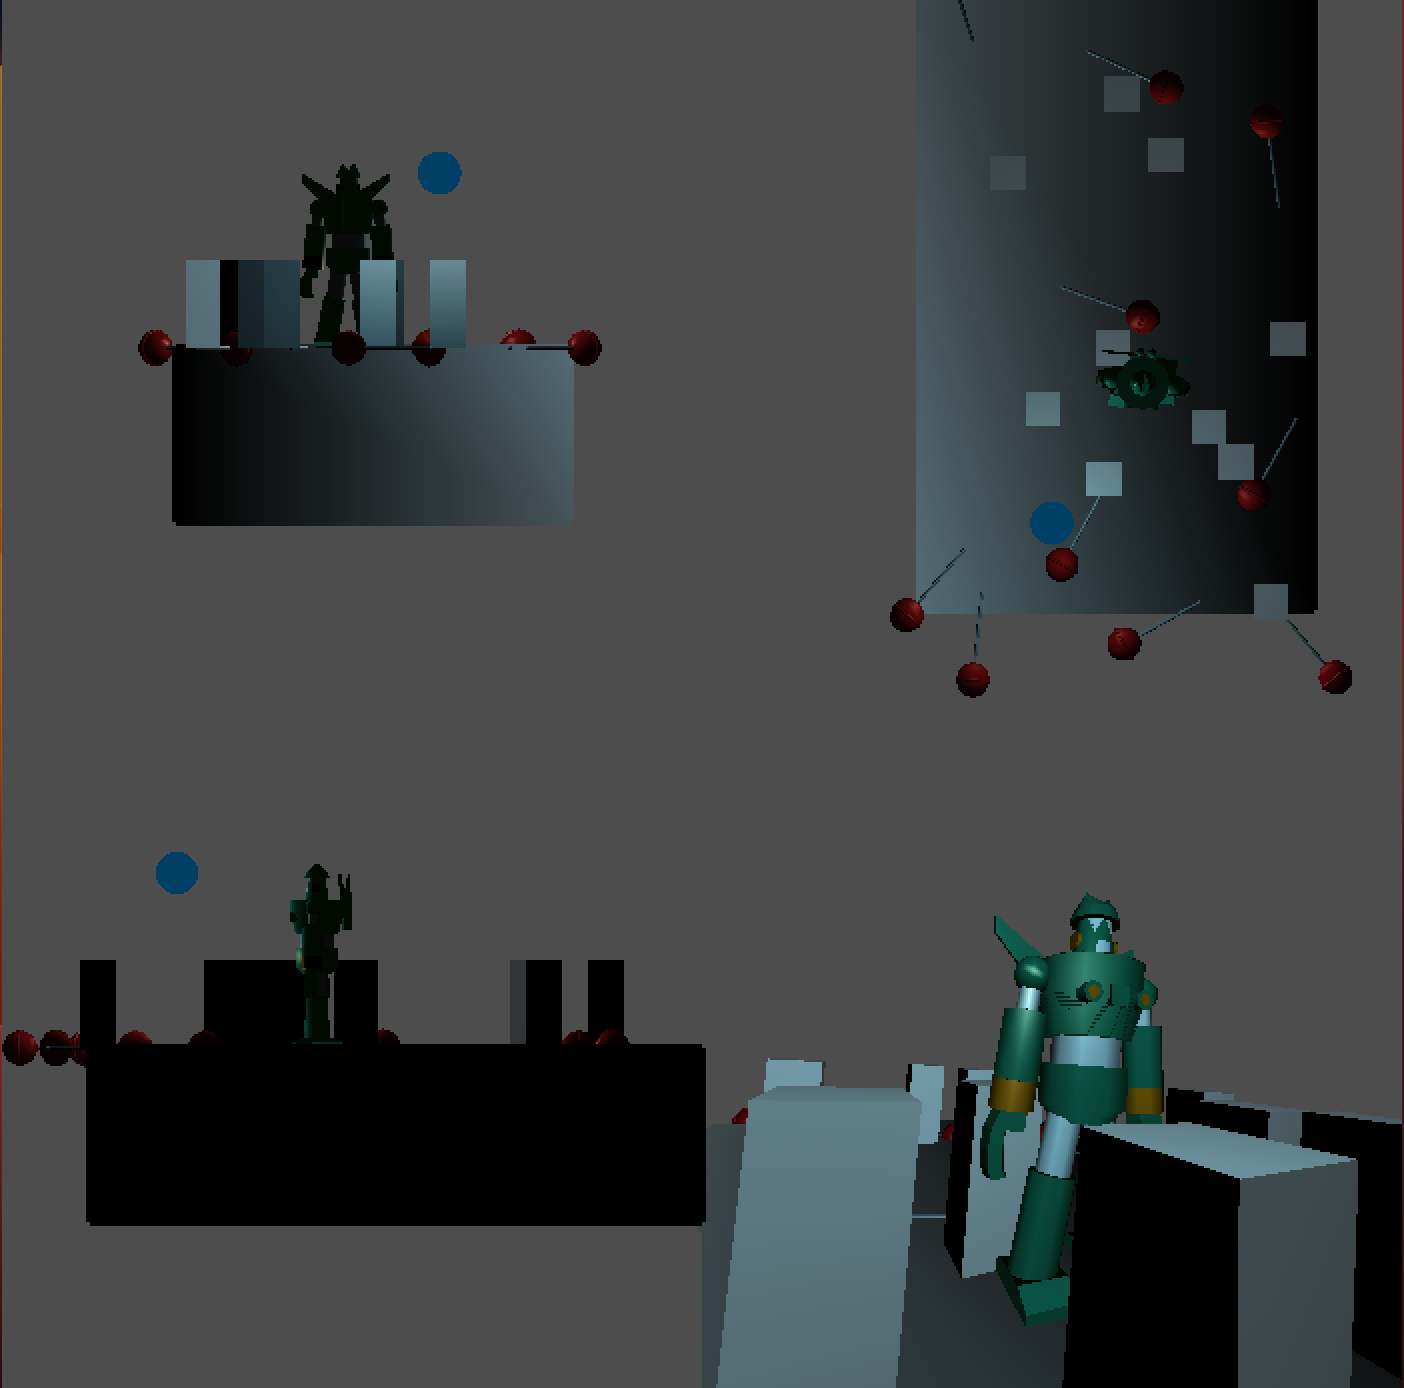
\includegraphics[scale=0.28]{pic2.png}

        \columnbreak

        開聚光燈的畫面

        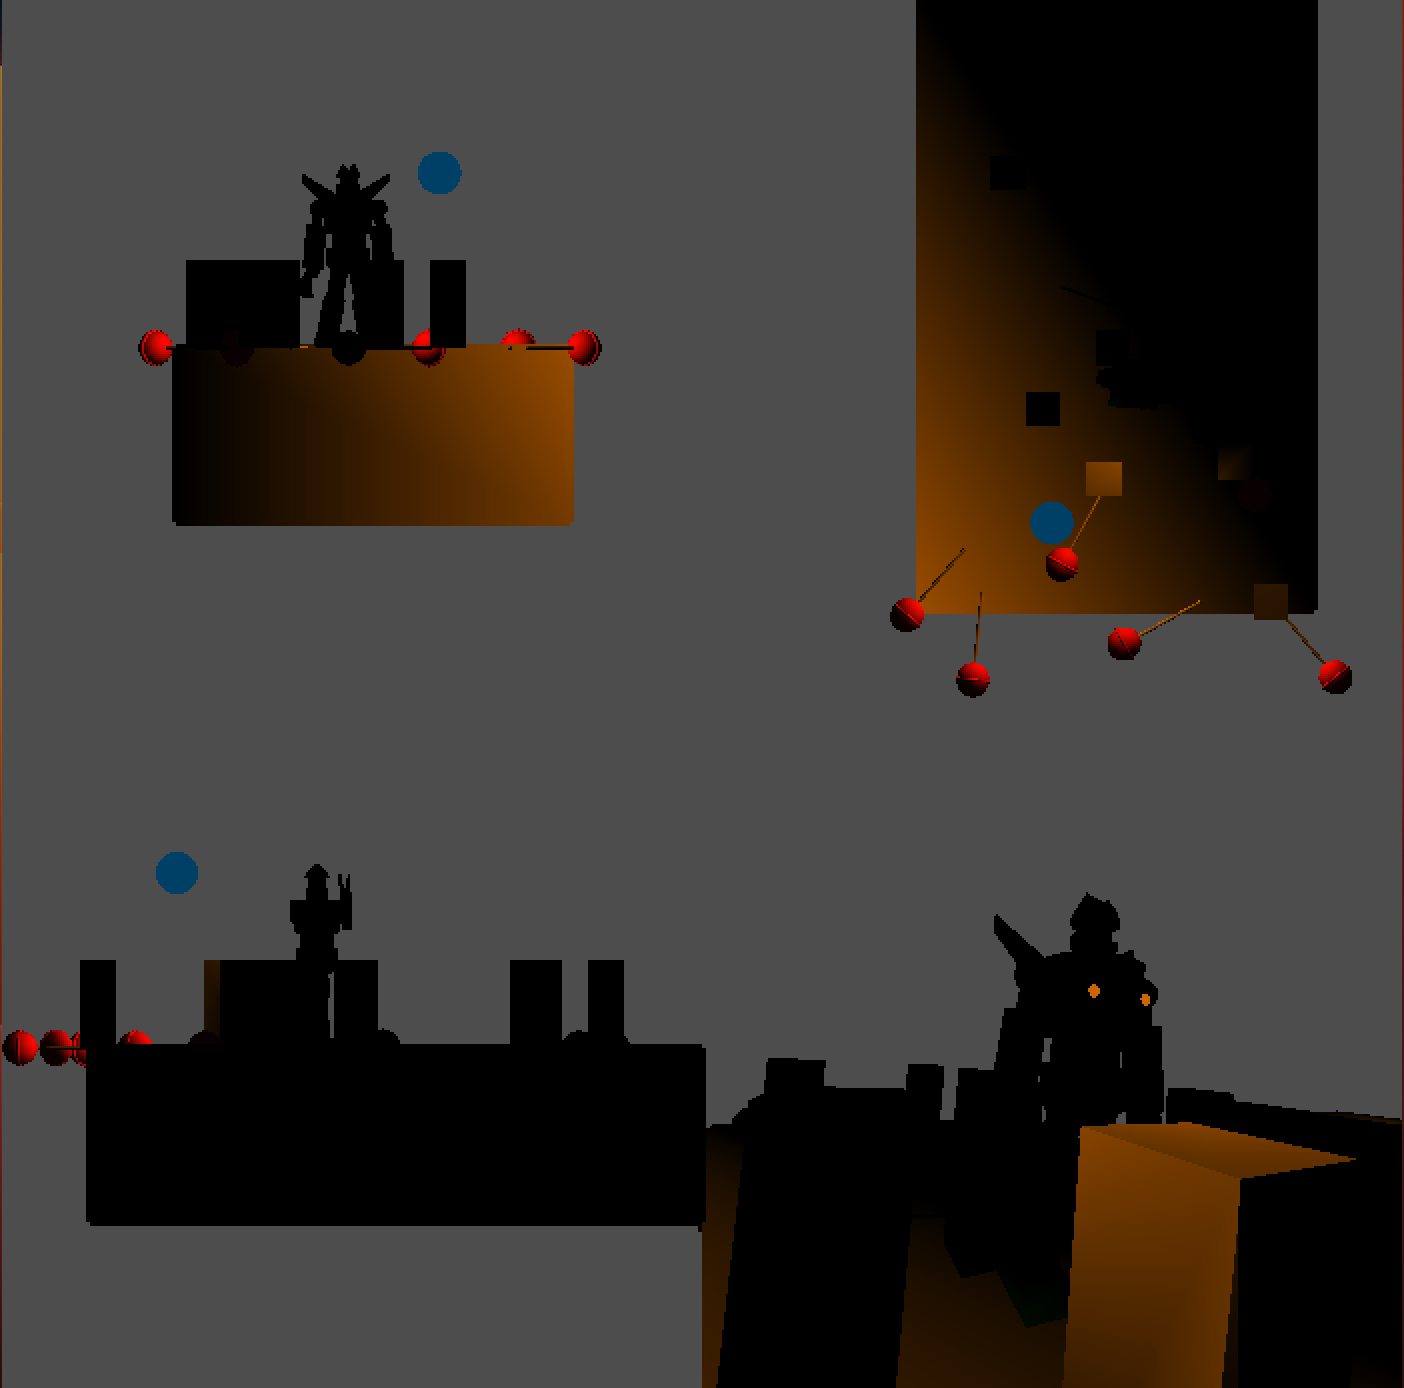
\includegraphics[scale=0.28]{pic3.png}

    \end{multicols}

\end{document}